% Options for packages loaded elsewhere
\PassOptionsToPackage{unicode}{hyperref}
\PassOptionsToPackage{hyphens}{url}
\PassOptionsToPackage{dvipsnames,svgnames,x11names}{xcolor}
%
\documentclass[
]{article}

\usepackage{amsmath,amssymb}
\usepackage{iftex}
\ifPDFTeX
  \usepackage[T1]{fontenc}
  \usepackage[utf8]{inputenc}
  \usepackage{textcomp} % provide euro and other symbols
\else % if luatex or xetex
  \usepackage{unicode-math}
  \defaultfontfeatures{Scale=MatchLowercase}
  \defaultfontfeatures[\rmfamily]{Ligatures=TeX,Scale=1}
\fi
\usepackage{lmodern}
\ifPDFTeX\else  
    % xetex/luatex font selection
  \setmainfont[]{Latin Modern Roman}
  \setmathfont[]{Latin Modern Math}
\fi
% Use upquote if available, for straight quotes in verbatim environments
\IfFileExists{upquote.sty}{\usepackage{upquote}}{}
\IfFileExists{microtype.sty}{% use microtype if available
  \usepackage[]{microtype}
  \UseMicrotypeSet[protrusion]{basicmath} % disable protrusion for tt fonts
}{}
\makeatletter
\@ifundefined{KOMAClassName}{% if non-KOMA class
  \IfFileExists{parskip.sty}{%
    \usepackage{parskip}
  }{% else
    \setlength{\parindent}{0pt}
    \setlength{\parskip}{6pt plus 2pt minus 1pt}}
}{% if KOMA class
  \KOMAoptions{parskip=half}}
\makeatother
\usepackage{xcolor}
\ifLuaTeX
  \usepackage{luacolor}
  \usepackage[soul]{lua-ul}
\else
  \usepackage{soul}
  
\fi
\setlength{\emergencystretch}{3em} % prevent overfull lines
\setcounter{secnumdepth}{5}
% Make \paragraph and \subparagraph free-standing
\ifx\paragraph\undefined\else
  \let\oldparagraph\paragraph
  \renewcommand{\paragraph}[1]{\oldparagraph{#1}\mbox{}}
\fi
\ifx\subparagraph\undefined\else
  \let\oldsubparagraph\subparagraph
  \renewcommand{\subparagraph}[1]{\oldsubparagraph{#1}\mbox{}}
\fi


\providecommand{\tightlist}{%
  \setlength{\itemsep}{0pt}\setlength{\parskip}{0pt}}\usepackage{longtable,booktabs,array}
\usepackage{calc} % for calculating minipage widths
% Correct order of tables after \paragraph or \subparagraph
\usepackage{etoolbox}
\makeatletter
\patchcmd\longtable{\par}{\if@noskipsec\mbox{}\fi\par}{}{}
\makeatother
% Allow footnotes in longtable head/foot
\IfFileExists{footnotehyper.sty}{\usepackage{footnotehyper}}{\usepackage{footnote}}
\makesavenoteenv{longtable}
\usepackage{graphicx}
\makeatletter
\def\maxwidth{\ifdim\Gin@nat@width>\linewidth\linewidth\else\Gin@nat@width\fi}
\def\maxheight{\ifdim\Gin@nat@height>\textheight\textheight\else\Gin@nat@height\fi}
\makeatother
% Scale images if necessary, so that they will not overflow the page
% margins by default, and it is still possible to overwrite the defaults
% using explicit options in \includegraphics[width, height, ...]{}
\setkeys{Gin}{width=\maxwidth,height=\maxheight,keepaspectratio}
% Set default figure placement to htbp
\makeatletter
\def\fps@figure{htbp}
\makeatother
% definitions for citeproc citations
\NewDocumentCommand\citeproctext{}{}
\NewDocumentCommand\citeproc{mm}{%
  \begingroup\def\citeproctext{#2}\cite{#1}\endgroup}
\makeatletter
 % allow citations to break across lines
 \let\@cite@ofmt\@firstofone
 % avoid brackets around text for \cite:
 \def\@biblabel#1{}
 \def\@cite#1#2{{#1\if@tempswa , #2\fi}}
\makeatother
\newlength{\cslhangindent}
\setlength{\cslhangindent}{1.5em}
\newlength{\csllabelwidth}
\setlength{\csllabelwidth}{3em}
\newenvironment{CSLReferences}[2] % #1 hanging-indent, #2 entry-spacing
 {\begin{list}{}{%
  \setlength{\itemindent}{0pt}
  \setlength{\leftmargin}{0pt}
  \setlength{\parsep}{0pt}
  % turn on hanging indent if param 1 is 1
  \ifodd #1
   \setlength{\leftmargin}{\cslhangindent}
   \setlength{\itemindent}{-1\cslhangindent}
  \fi
  % set entry spacing
  \setlength{\itemsep}{#2\baselineskip}}}
 {\end{list}}
\usepackage{calc}
\newcommand{\CSLBlock}[1]{\hfill\break\parbox[t]{\linewidth}{\strut\ignorespaces#1\strut}}
\newcommand{\CSLLeftMargin}[1]{\parbox[t]{\csllabelwidth}{\strut#1\strut}}
\newcommand{\CSLRightInline}[1]{\parbox[t]{\linewidth - \csllabelwidth}{\strut#1\strut}}
\newcommand{\CSLIndent}[1]{\hspace{\cslhangindent}#1}

\usepackage{arxiv}
\usepackage{orcidlink}
\usepackage{amsmath}
\usepackage[T1]{fontenc}
\makeatletter
\@ifpackageloaded{caption}{}{\usepackage{caption}}
\AtBeginDocument{%
\ifdefined\contentsname
  \renewcommand*\contentsname{Table of contents}
\else
  \newcommand\contentsname{Table of contents}
\fi
\ifdefined\listfigurename
  \renewcommand*\listfigurename{List of Figures}
\else
  \newcommand\listfigurename{List of Figures}
\fi
\ifdefined\listtablename
  \renewcommand*\listtablename{List of Tables}
\else
  \newcommand\listtablename{List of Tables}
\fi
\ifdefined\figurename
  \renewcommand*\figurename{Figure}
\else
  \newcommand\figurename{Figure}
\fi
\ifdefined\tablename
  \renewcommand*\tablename{Table}
\else
  \newcommand\tablename{Table}
\fi
}
\@ifpackageloaded{float}{}{\usepackage{float}}
\floatstyle{ruled}
\@ifundefined{c@chapter}{\newfloat{codelisting}{h}{lop}}{\newfloat{codelisting}{h}{lop}[chapter]}
\floatname{codelisting}{Listing}
\newcommand*\listoflistings{\listof{codelisting}{List of Listings}}
\makeatother
\makeatletter
\makeatother
\makeatletter
\@ifpackageloaded{caption}{}{\usepackage{caption}}
\@ifpackageloaded{subcaption}{}{\usepackage{subcaption}}
\makeatother
\ifLuaTeX
  \usepackage{selnolig}  % disable illegal ligatures
\fi
\usepackage{bookmark}

\IfFileExists{xurl.sty}{\usepackage{xurl}}{} % add URL line breaks if available
\urlstyle{same} % disable monospaced font for URLs
\hypersetup{
  pdftitle={Comparison of Catalogs},
  colorlinks=true,
  linkcolor={blue},
  filecolor={Maroon},
  citecolor={Blue},
  urlcolor={Blue},
  pdfcreator={LaTeX via pandoc}}

\newcommand{\runninghead}{A Preprint }
\title{Comparison of Catalogs}
\def\asep{\\\\\\ } % default: all authors on same column
\author{}
\date{}
\begin{document}
\maketitle

\renewcommand*\contentsname{Table of contents}
{
\hypersetup{linkcolor=}
\setcounter{tocdepth}{3}
\tableofcontents
}
\section{The data}\label{the-data}

In this script we will compare 2 catalogs Kovlakas et al. (2021) and
Karachentsev and Kaisina (2013)

\begin{itemize}
\tightlist
\item
  The data have been joined based on their position in the sky (Ra,
  Dec).

  \begin{itemize}
  \tightlist
  \item
    We assume that every galaxy within 2 arc seconds of the initial
    coordinates is the same galaxy.
  \end{itemize}
\item
  We use TOPCAT to create two joins, an inner and an outer join
\item
  We will use the inner join for 1-1 comparisons
\item
  If we see that the data are similar we can use the outer join
\item
  For the comparison we keep the parameters names exactly they are given
  in the catalogs
\end{itemize}

The dataset we are going to use for the comparison (inner join) consists
of 288 galaxies and 168 columns.

\section{Catalog Completeness}\label{catalog-completeness}

Checking for completeness in galaxy catalogs is essential to ensure that
the data accurately represents the true population of galaxies.
Incomplete catalogs can lead to biased results in statistical studies,
such as the distribution of galaxy luminosity, mass, or star formation
rates. Additionally, missing galaxies, especially those at faint
magnitudes or large distances, can distort cosmological measurements and
hinder our understanding of galaxy formation and evolution.

Completeness checks are crucial for addressing selection biases,
ensuring accurate redshift distributions, and validating galaxy
simulations. They help identify gaps in the data and guide follow-up
observations, ensuring that the catalog provides a reliable sample for
scientific analysis. Without these checks, conclusions drawn from the
data may be inaccurate or incomplete.

\begin{center}\rule{0.5\linewidth}{0.5pt}\end{center}

Checking for completeness in galaxy catalogs is essential to ensure that
the data accurately represents the true population of galaxies.
Incomplete catalogs can lead to biased results in statistical studies,
such as the distribution of galaxy luminosity, mass, or star formation
rates. Additionally, missing galaxies, especially those at faint
magnitudes or large distances, can distort cosmological measurements and
hinder our understanding of galaxy formation and evolution. Completeness
checks are crucial for addressing selection biases, ensuring accurate
redshift distributions, and validating galaxy simulations.

Distance-based corrections are applied to mitigate these biases by
adjusting for the underrepresentation of galaxies at greater distances.
As galaxies move farther away, they become fainter and harder to detect,
leading to a drop in the number of detected galaxies. Methods like
\textbf{volume corrections} (e.g., V/Vmax) and \textbf{luminosity
function-based corrections} help account for these effects by estimating
the true galaxy population based on the observed sample. These
corrections ensure that statistical analyses, even in incomplete
catalogs, more accurately reflect the full galaxy population.

\begin{longtable}[]{@{}lr@{}}
\toprule\noalign{}
Table & Number of galaxies \\
\midrule\noalign{}
\endhead
\bottomrule\noalign{}
\endlastfoot
Inner join & 288 \\
Outer join & 2901 \\
LCV & 1316 \\
HECATE & 2901 \\
Unique galaxies in LCV & 1028 \\
Unique Galaxies in Hecate & 2613 \\
\end{longtable}

\subsection{Completeness of the Inner
join}\label{completeness-of-the-inner-join}

\[
\text{Completeness (X)}=\frac{\text{(Galaxies in Inner Join)}}{\text{(Galaxies in X)}}×100\%
\]

Completeness (HECATE)= 10 \%

Completeness (LCV)= 22 \%

\subsection{Completeness in Outer
join}\label{completeness-in-outer-join}

\[
\text{Completeness (X)}=\frac{\text{(Galaxies in Outer Join form X)}}{\text{(Galaxies in X)}}×100\%
\]

Completeness (HECATE)= 90 \%

Completeness (LCV)= 78 \%

Combined Completeness
=\(\frac{\text{Total galaxies in Outer}}{\text{Unique galaxies in HECATE + LCV}}\)=
80 \%

\subsection{Completeness of the Catalogs, based on the Distance and the
Morphological
Type}\label{completeness-of-the-catalogs-based-on-the-distance-and-the-morphological-type}

\begin{figure}

\begin{minipage}{0.50\linewidth}

\centering{

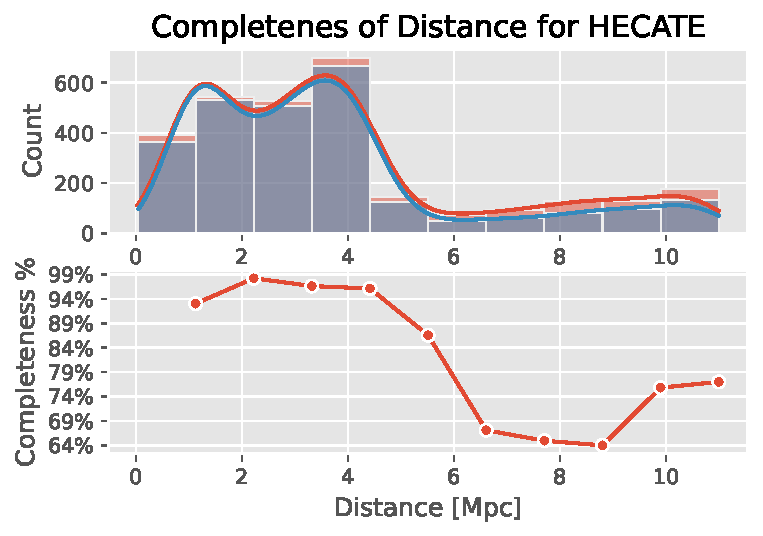
\includegraphics{compare_files/figure-pdf/fig-dis-comp-output-1.pdf}

}

\subcaption{\label{fig-dis-comp-1}HECATE}

\end{minipage}%
%
\begin{minipage}{0.50\linewidth}

\centering{

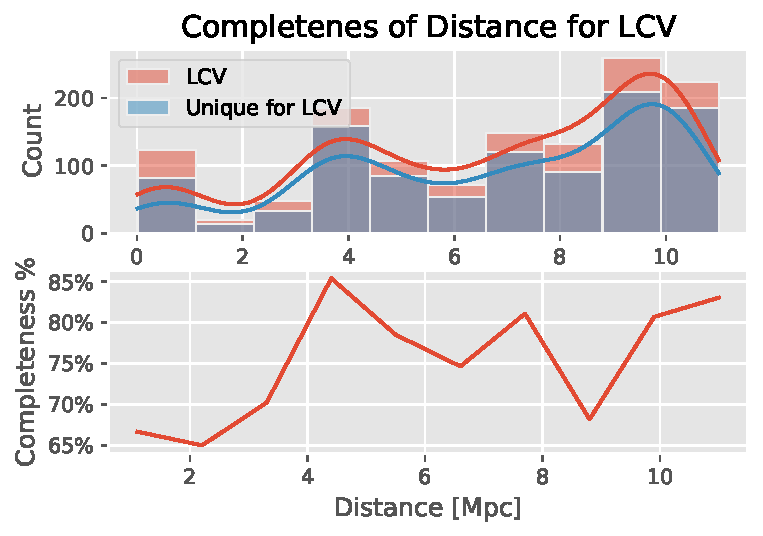
\includegraphics{compare_files/figure-pdf/fig-dis-comp-output-2.pdf}

}

\subcaption{\label{fig-dis-comp-2}LCV}

\end{minipage}%

\caption{\label{fig-dis-comp}Histograms showing the Completeness of the
Catalogs}

\end{figure}%

\begin{figure}

\begin{minipage}{0.50\linewidth}

\centering{

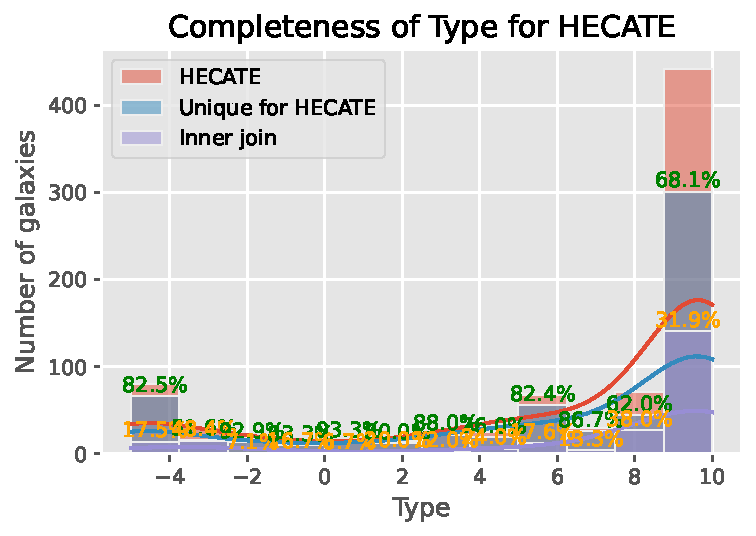
\includegraphics{compare_files/figure-pdf/fig-type-comp-output-1.pdf}

}

\subcaption{\label{fig-type-comp-1}HECATE}

\end{minipage}%
%
\begin{minipage}{0.50\linewidth}

\centering{

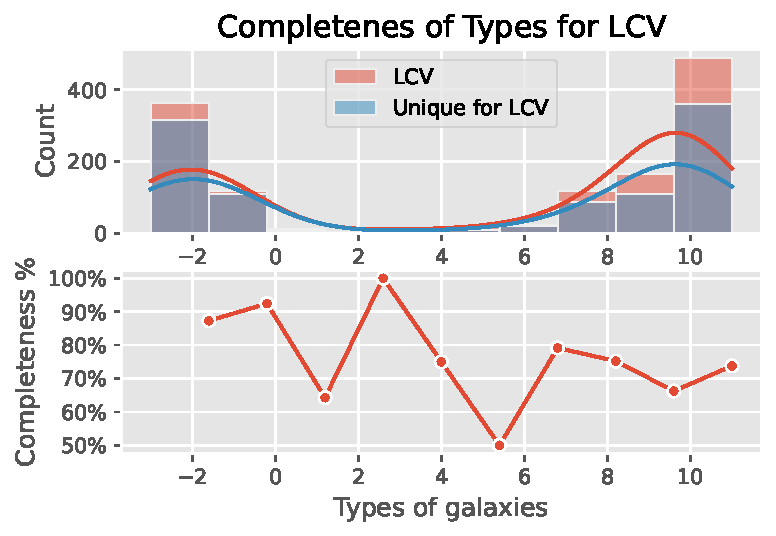
\includegraphics{compare_files/figure-pdf/fig-type-comp-output-2.pdf}

}

\subcaption{\label{fig-type-comp-2}LCV}

\end{minipage}%

\caption{\label{fig-type-comp}Histograms showing the Completeness of the
Catalogs}

\end{figure}%

\begin{figure}

\begin{minipage}{0.50\linewidth}

\begin{longtable}[]{@{}rr@{}}
\toprule\noalign{}
Value & Count \\
\midrule\noalign{}
\endhead
\bottomrule\noalign{}
\endlastfoot
-3 & 138 \\
-2 & 224 \\
-1 & 119 \\
0 & 4 \\
1 & 7 \\
2 & 2 \\
3 & 8 \\
4 & 9 \\
5 & 7 \\
6 & 24 \\
7 & 31 \\
8 & 86 \\
9 & 166 \\
10 & 484 \\
11 & 4 \\
\end{longtable}

\end{minipage}%
%
\begin{minipage}{0.50\linewidth}

\begin{longtable}[]{@{}rr@{}}
\toprule\noalign{}
Value & Count \\
\midrule\noalign{}
\endhead
\bottomrule\noalign{}
\endlastfoot
-5 & 52 \\
-4.9 & 7 \\
-4.8 & 13 \\
-4.7 & 2 \\
-4.3 & 2 \\
-4 & 3 \\
-3.9 & 1 \\
-3.7 & 1 \\
-3.5 & 3 \\
-3.3 & 1 \\
-3.1 & 1 \\
-3 & 11 \\
-2.9 & 3 \\
-2.8 & 3 \\
-2.7 & 3 \\
-2.6 & 5 \\
-2.5 & 1 \\
-2.1 & 2 \\
-2 & 3 \\
-1.9 & 1 \\
-1.8 & 3 \\
-1.7 & 1 \\
-1.6 & 1 \\
-1.3 & 2 \\
-1 & 8 \\
-0.8 & 1 \\
-0.4 & 2 \\
-0.1 & 1 \\
0 & 3 \\
0.1 & 1 \\
0.4 & 1 \\
0.5 & 1 \\
0.6 & 1 \\
1 & 5 \\
1.1 & 2 \\
1.2 & 1 \\
1.3 & 1 \\
1.5 & 2 \\
1.6 & 2 \\
1.8 & 1 \\
1.9 & 2 \\
2.1 & 1 \\
2.2 & 2 \\
2.3 & 1 \\
2.4 & 3 \\
2.5 & 1 \\
2.6 & 1 \\
2.7 & 1 \\
2.9 & 1 \\
3 & 3 \\
3.1 & 4 \\
3.2 & 1 \\
3.3 & 6 \\
3.4 & 3 \\
3.5 & 2 \\
3.6 & 2 \\
3.8 & 2 \\
3.9 & 2 \\
4 & 13 \\
4.1 & 1 \\
4.2 & 2 \\
4.4 & 2 \\
4.5 & 1 \\
4.7 & 1 \\
4.8 & 1 \\
5 & 21 \\
5.1 & 5 \\
5.2 & 5 \\
5.3 & 1 \\
5.4 & 3 \\
5.5 & 1 \\
5.7 & 1 \\
5.8 & 2 \\
5.9 & 9 \\
6 & 13 \\
6.1 & 7 \\
6.4 & 1 \\
6.5 & 2 \\
6.7 & 3 \\
6.8 & 2 \\
6.9 & 5 \\
7 & 11 \\
7.1 & 1 \\
7.2 & 2 \\
7.3 & 1 \\
7.4 & 2 \\
7.5 & 4 \\
7.6 & 1 \\
7.7 & 3 \\
7.8 & 6 \\
7.9 & 9 \\
8 & 19 \\
8.1 & 4 \\
8.2 & 3 \\
8.3 & 5 \\
8.4 & 2 \\
8.5 & 4 \\
8.6 & 5 \\
8.7 & 6 \\
8.8 & 9 \\
8.9 & 15 \\
9 & 29 \\
9.1 & 4 \\
9.2 & 4 \\
9.3 & 2 \\
9.4 & 4 \\
9.5 & 13 \\
9.6 & 4 \\
9.7 & 17 \\
9.8 & 48 \\
9.9 & 90 \\
10 & 203 \\
\end{longtable}

\end{minipage}%

\end{figure}%

As we can see from the histograms Figure~\ref{fig-dis-comp} and
Figure~\ref{fig-type-comp} the sample of nique galaxies of each catalog,
gets smaller by an almost constant proportion (Inner join).

This means there is no bias in the selection of the galaxies.

\section{How are we going to compare the
data?}\label{how-are-we-going-to-compare-the-data}

\subsection{\texorpdfstring{Scatter plots and \(R^2\)
calculation}{Scatter plots and R\^{}2 calculation}}\label{scatter-plots-and-r2-calculation}

\begin{enumerate}
\def\labelenumi{\arabic{enumi}.}
\tightlist
\item
  \(R^2\): Measures the proportion of variance explained by the linear
  model.
\item
  Slope of the Fitted Line: Should be close to 1 for a 1-1
  correlation.\footnote{Some data seem to have a very good linear
    correlation but they have many outliers. This is why we will clip
    the outliers with \(\sigma > 3\)}
\end{enumerate}

\begin{enumerate}
\def\labelenumi{\arabic{enumi}.}
\setcounter{enumi}{2}
\tightlist
\item
  Pearson Correlation \(\rho\): Measures the strength and direction of
  the linear relationship between two variables, ranging from -1 to 1.
  \footnote{In simple linear regression, \(R^2\) is the square of the
    Pearson correlation coefficient \(\rho\).}
\end{enumerate}

\begin{enumerate}
\def\labelenumi{\arabic{enumi}.}
\setcounter{enumi}{3}
\tightlist
\item
  \ul{Plots}: Plots are essential for visually assessing the
  relationship between two datasets, identifying correlations, trends,
  and outliers, and evaluating the fit of linear models.
\end{enumerate}

\begin{itemize}
\tightlist
\item
  Histograms: Because not all of our data have the same number of
  counts, the comparison with histograms between data that are not the
  same, doesn't help us right now.\footnote{When we will use the outer
    join table we could use histograms due to the large number of
    counts.} This is why we will only use histograms for comparing the
  distribution of same-data columns normalized by their maximum value
\end{itemize}

\begin{itemize}
\item
  Correlation Heatmaps: A correlation heatmap is a graphical tool that
  displays the correlation between multiple variables as a color-coded
  matrix. It's like a color chart that shows us how closely related
  different variables are. In a correlation heatmap, each variable is
  represented by a row and a column, and the cells show the correlation
  between them. The color of each cell represents the strength and
  direction of the correlation, with darker colors indicating stronger
  correlations.
\item
  Kernel Density Estimate (KDE) plot: The KDE plot visually represents
  the distribution of data, providing insights into its shape, central
  tendency, and spread.
\end{itemize}

\begin{enumerate}
\def\labelenumi{\arabic{enumi}.}
\setcounter{enumi}{4}
\tightlist
\item
  Percentage change: We can calculate the percentage change of the data
  for each galaxy and then we can see if the data are similar, based on
  minimum, the maximum and the mean value of the difference.
\end{enumerate}

\[\text{Percentage change} = \frac{V_{Hecate} - V_{LCV}}{V_{Hecate}}\cdot 100 \%\]

\section{Comparable data}\label{comparable-data}

\subsection{Coordinates}\label{coordinates}

\begin{longtable}[]{@{}cccc@{}}
\toprule\noalign{}
LCV & HECATE & Description & Pearson Correlation {[}-1,1{]} \\
\midrule\noalign{}
\endhead
\bottomrule\noalign{}
\endlastfoot
Ra\_1 & RA\_2 & Right Ascension & 1.0 \\
Dec\_1 & DEC\_2 & Declination & 1.0 \\
Dis & D & Distance & 0.881 \\
\end{longtable}

\subsubsection{Right Ascension}

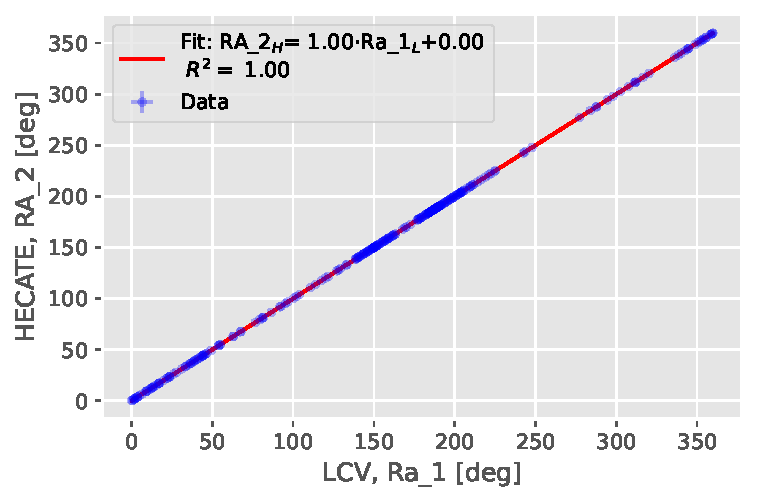
\includegraphics{compare_files/figure-pdf/cell-12-output-1.pdf}

\subsubsection{Declination}

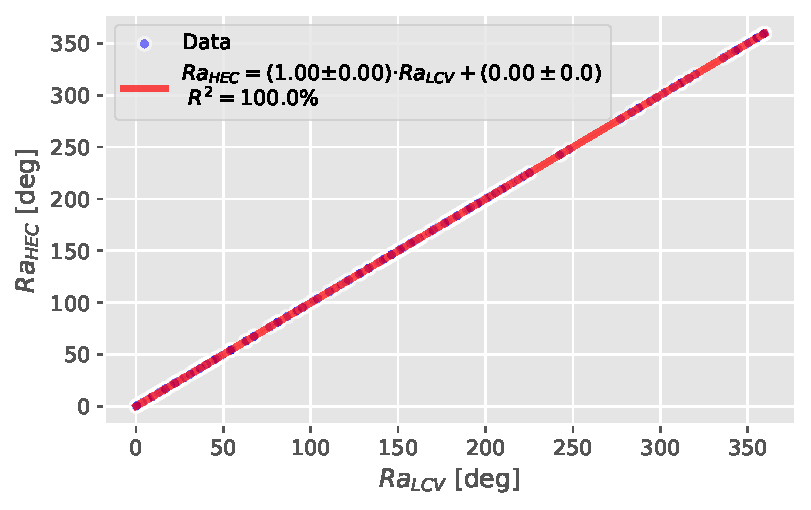
\includegraphics{compare_files/figure-pdf/cell-13-output-1.pdf}

\subsubsection{Distance}

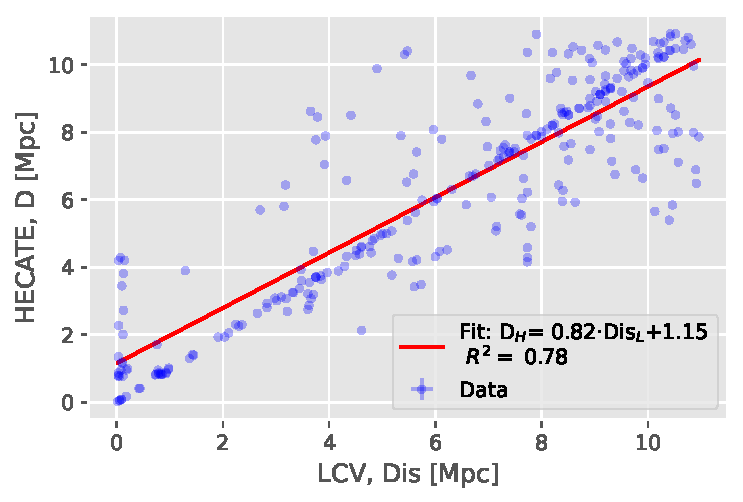
\includegraphics{compare_files/figure-pdf/cell-14-output-1.pdf}

\subsection{Velocities}\label{velocities}

\begin{longtable}[]{@{}
  >{\centering\arraybackslash}p{(\columnwidth - 6\tabcolsep) * \real{0.2466}}
  >{\centering\arraybackslash}p{(\columnwidth - 6\tabcolsep) * \real{0.2603}}
  >{\centering\arraybackslash}p{(\columnwidth - 6\tabcolsep) * \real{0.2466}}
  >{\centering\arraybackslash}p{(\columnwidth - 6\tabcolsep) * \real{0.2466}}@{}}
\toprule\noalign{}
\begin{minipage}[b]{\linewidth}\centering
LCV
\end{minipage} & \begin{minipage}[b]{\linewidth}\centering
HECATE
\end{minipage} & \begin{minipage}[b]{\linewidth}\centering
Description
\end{minipage} & \begin{minipage}[b]{\linewidth}\centering
Linear Correlation
\end{minipage} \\
\midrule\noalign{}
\endhead
\bottomrule\noalign{}
\endlastfoot
RVel (km/s) & V (km/s) & Heliocentric radial velocity & 0.994 \\
VLG (km/s) & & Radial velocity & \\
cz (km/s) & & Heliocentric velocity & \\
& V\_VIR (km/s) & Virgo-infall corrected radial velocity & \\
\end{longtable}

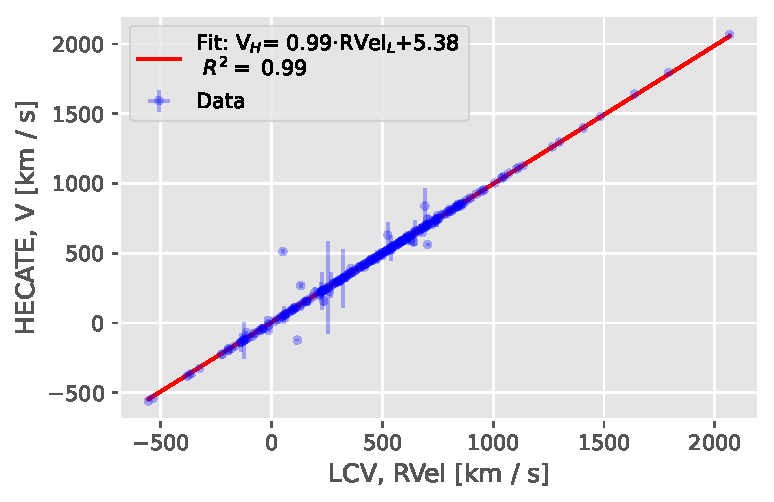
\includegraphics{compare_files/figure-pdf/cell-16-output-1.pdf}

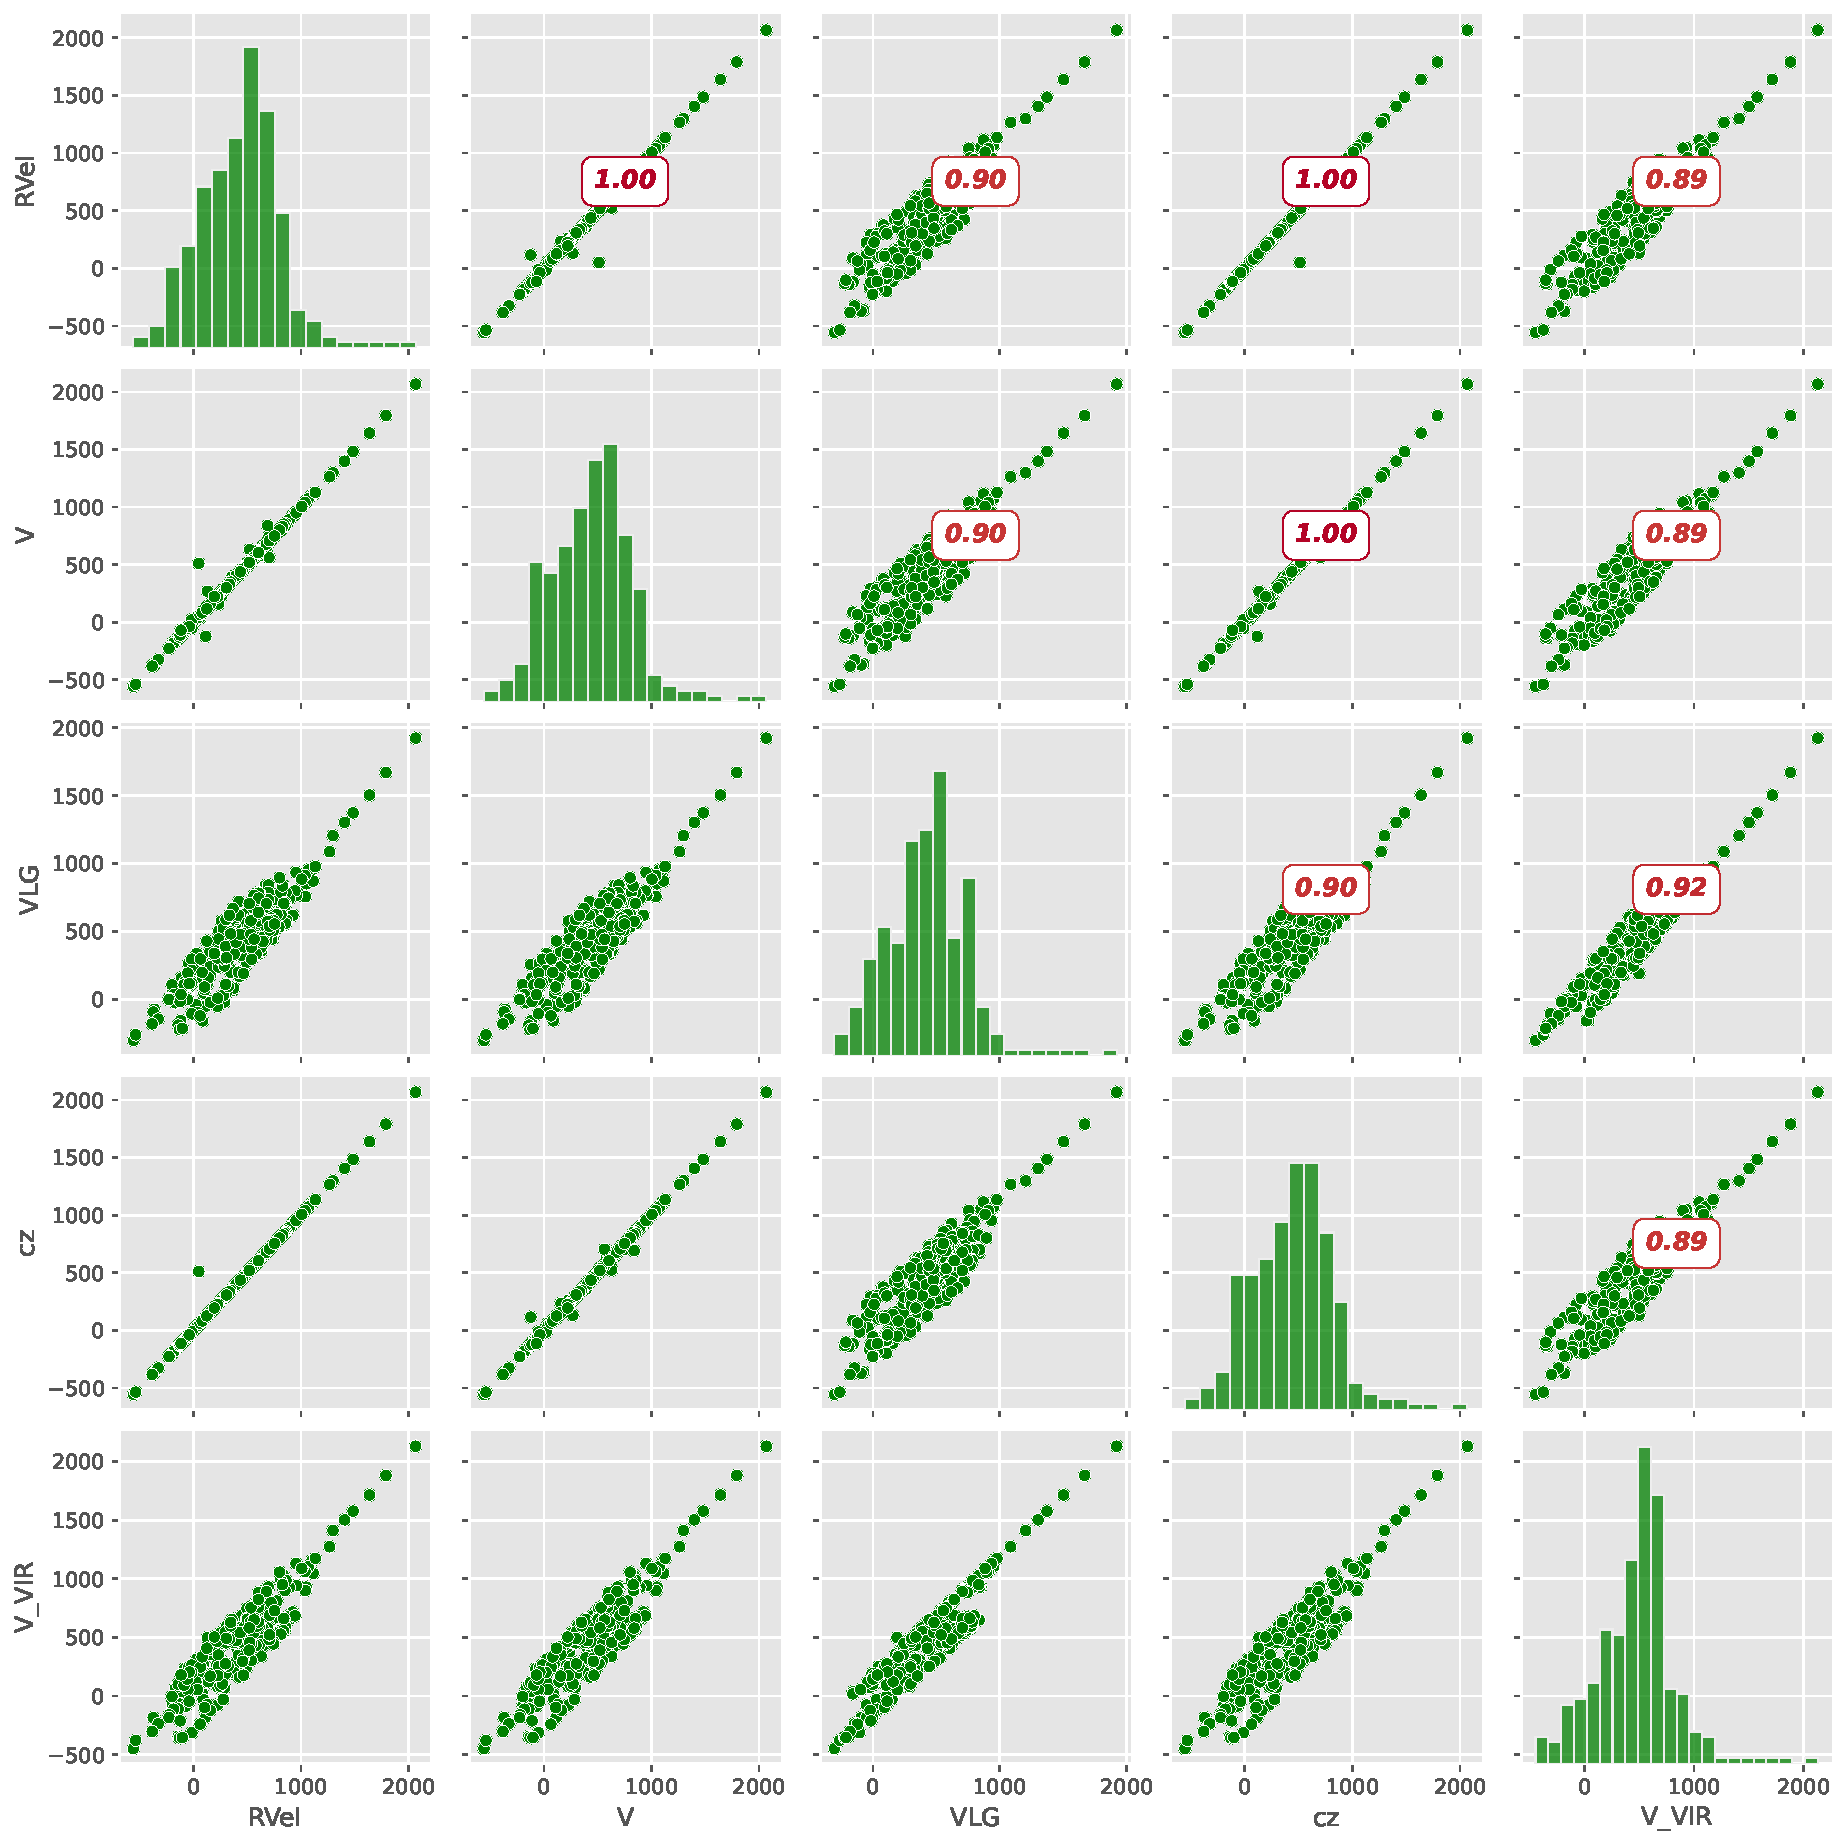
\includegraphics{compare_files/figure-pdf/cell-18-output-1.pdf}

{[}?{]} The close correlation between all of the velocities, could be
due to the fact that all of them measure the velocity of each galaxy,
but from a different frame of reference.

\subsection{Morphology and Geometry}\label{morphology-and-geometry}

\begin{longtable}[]{@{}
  >{\centering\arraybackslash}p{(\columnwidth - 6\tabcolsep) * \real{0.2466}}
  >{\centering\arraybackslash}p{(\columnwidth - 6\tabcolsep) * \real{0.2466}}
  >{\centering\arraybackslash}p{(\columnwidth - 6\tabcolsep) * \real{0.2603}}
  >{\centering\arraybackslash}p{(\columnwidth - 6\tabcolsep) * \real{0.2466}}@{}}
\toprule\noalign{}
\begin{minipage}[b]{\linewidth}\centering
LCV
\end{minipage} & \begin{minipage}[b]{\linewidth}\centering
HECATE
\end{minipage} & \begin{minipage}[b]{\linewidth}\centering
Description
\end{minipage} & \begin{minipage}[b]{\linewidth}\centering
Pearson Correlation {[}-1,1{]}
\end{minipage} \\
\midrule\noalign{}
\endhead
\bottomrule\noalign{}
\endlastfoot
TType & T (with errors) & Numerical Hubble type following the de
Vaucouleurs system & 0.7107 \\
inc & INCL & Inclination (deg) & 0 \\
a26\_1 (Major) & R1 (Semi-major axis) & angular diameter (arcmin) & 0 \\
\end{longtable}

\subsubsection{Galaxy Types}

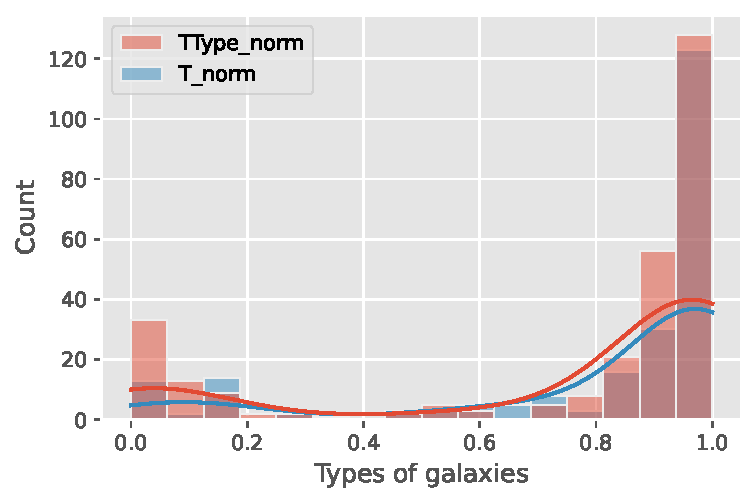
\includegraphics{compare_files/figure-pdf/cell-21-output-1.pdf}

\textbf{Percentage change:}

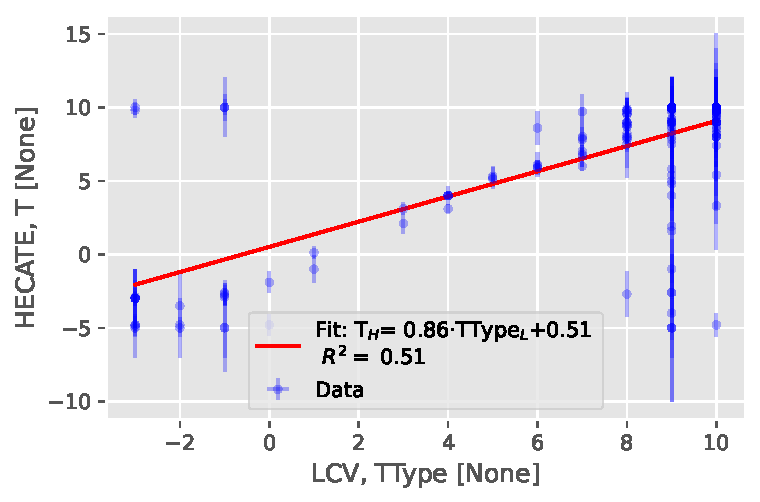
\includegraphics{compare_files/figure-pdf/cell-22-output-1.pdf}

\begin{longtable}[]{@{}lll@{}}
\toprule\noalign{}
& diff\_T & diff\_T\_clip \\
\midrule\noalign{}
\endhead
\bottomrule\noalign{}
\endlastfoot
count & 229 & 191 \\
mean & -30 & -1 \\
std & 119 & 10 \\
min & -1000 & -39 \\
25\% & -11 & -2 \\
50\% & 0 & 0 \\
75\% & 0 & 2 \\
max & 131 & 30 \\
\end{longtable}

{[}?{]} After the sigma clip we only lose 39 galaxies (\(14\%\)) and we
can see that both the median and the mean of the percentage change are
close to \(0\%\).This is why we can assume that the Types of the
galaxies are the same for the two catalogs

\paragraph{Normalize the scale of galaxy
types}\label{normalize-the-scale-of-galaxy-types}

It is very possible that the two catalogs use different scaling methods,
as indicated by the use of decimal numbers in HECATE.

\begin{longtable}[]{@{}lllll@{}}
\toprule\noalign{}
& T & TType & T\_norm & TType\_norm \\
\midrule\noalign{}
\endhead
\bottomrule\noalign{}
\endlastfoot
count & 229 & 287 & 229 & 287 \\
mean & 7 & 7 & 1 & 1 \\
std & 5 & 5 & 0 & 0 \\
min & -5 & -3 & 0 & 0 \\
25\% & 7 & 6 & 1 & 1 \\
50\% & 10 & 9 & 1 & 1 \\
75\% & 10 & 10 & 1 & 1 \\
max & 10 & 10 & 1 & 1 \\
\end{longtable}

Also, as we can see the minimum values are lower by 2 in HECATE, which
complies with the linear fit.

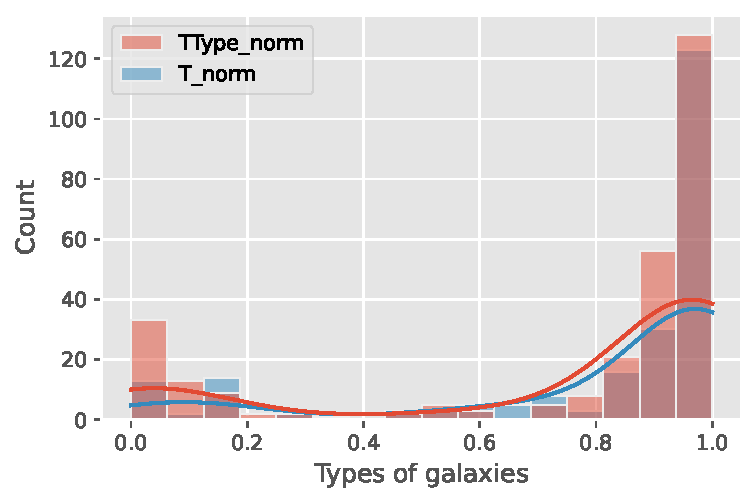
\includegraphics{compare_files/figure-pdf/cell-25-output-1.pdf}

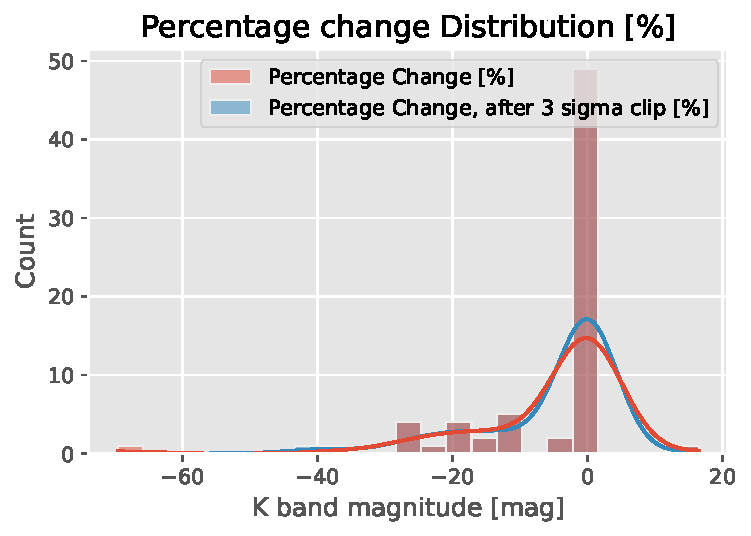
\includegraphics{compare_files/figure-pdf/cell-26-output-1.pdf}

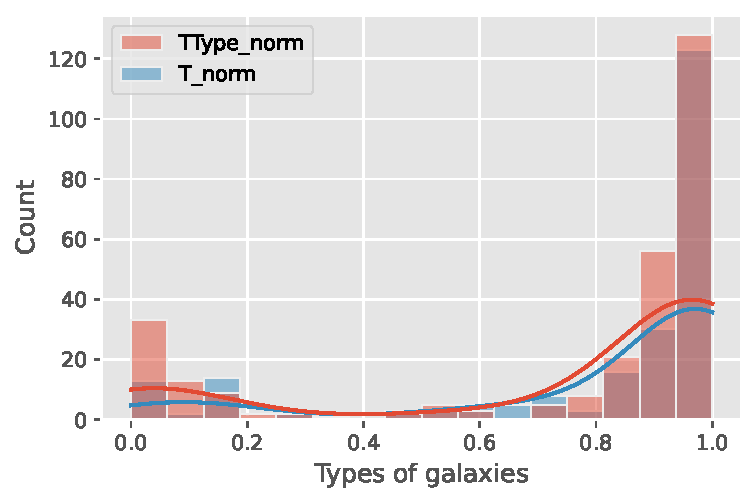
\includegraphics{compare_files/figure-pdf/cell-27-output-1.pdf}

\subsubsection{Inclination}

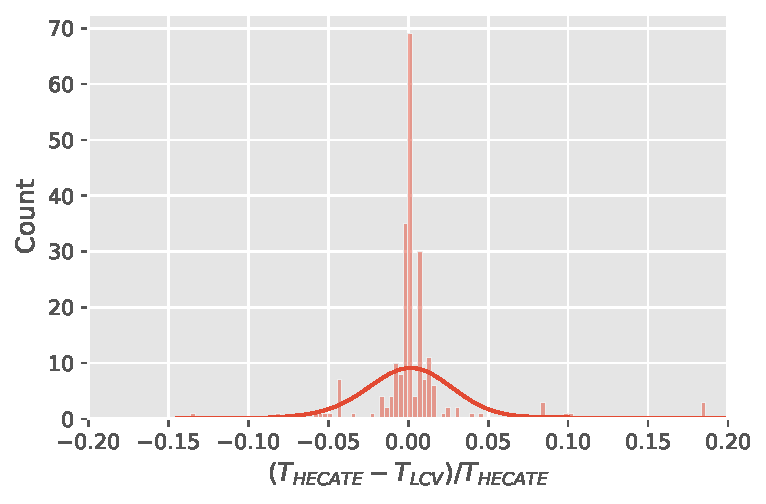
\includegraphics{compare_files/figure-pdf/cell-28-output-1.pdf}

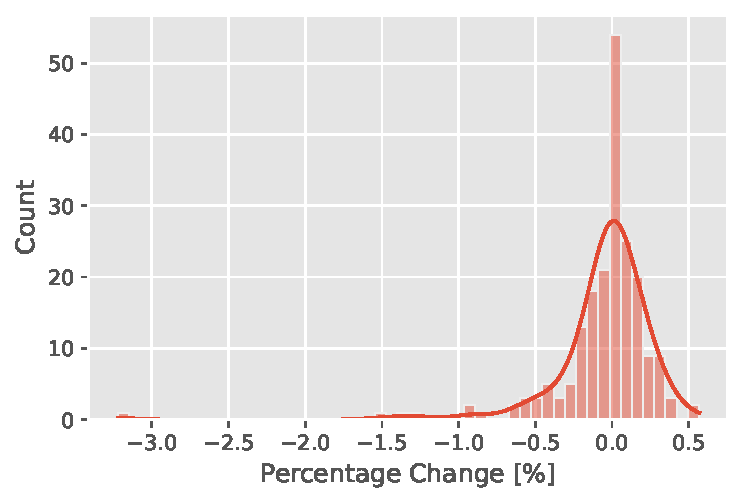
\includegraphics{compare_files/figure-pdf/cell-28-output-2.pdf}

\begin{longtable}[]{@{}llll@{}}
\toprule\noalign{}
& inc & INCL & Percentage Change {[}\%{]} \\
\midrule\noalign{}
\endhead
\bottomrule\noalign{}
\endlastfoot
count & 287 & 209 & 202 \\
mean & 60 & 59 & -0 \\
std & 19 & 23 & 0 \\
min & 9 & 0 & -3 \\
25\% & 47 & 47 & -0 \\
50\% & 60 & 59 & 0 \\
75\% & 72 & 78 & 0 \\
max & 90 & 90 & 1 \\
\end{longtable}

We can see that for values in the range
\([\sim 30^\circ,\sim 80^\circ]\), the values of the LCV inclination are
higher. However, since their means, median, min and maxes are similar
and the percentage change is practically 0\% (mean, median, \(\sigma\) =
0 with a range \([-3\%,1\%]\)), we can ignore the differences and assume
they are the same values.

\subsubsection{Major Axis}

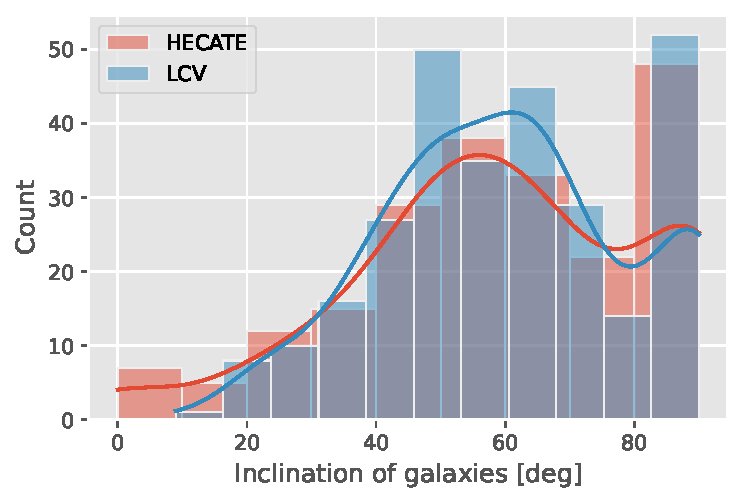
\includegraphics{compare_files/figure-pdf/cell-29-output-1.pdf}

it is not very clear if we truly have a correlation or not. We need to
see the linear correlation of the decimal logarithms.

\begin{verbatim}
 ** On entry to DLASCL parameter number  4 had an illegal value
 ** On entry to DLASCL parameter number  4 had an illegal value
 ** On entry to DLASCL parameter number  4 had an illegal value
 ** On entry to DLASCL parameter number  4 had an illegal value
 ** On entry to DLASCL parameter number  5 had an illegal value
 ** On entry to DLASCL parameter number  4 had an illegal value
 ** On entry to DLASCL parameter number  4 had an illegal value
 ** On entry to DLASCL parameter number  4 had an illegal value
 ** On entry to DLASCL parameter number  4 had an illegal value
 ** On entry to DLASCL parameter number  4 had an illegal value
 ** On entry to DLASCL parameter number  5 had an illegal value
 ** On entry to DLASCL parameter number  4 had an illegal value
 ** On entry to DLASCL parameter number  4 had an illegal value
 ** On entry to DLASCL parameter number  4 had an illegal value
 ** On entry to DLASCL parameter number  4 had an illegal value
 ** On entry to DLASCL parameter number  4 had an illegal value
 ** On entry to DLASCL parameter number  5 had an illegal value
 ** On entry to DLASCL parameter number  4 had an illegal value
 ** On entry to DLASCL parameter number  4 had an illegal value
 ** On entry to DLASCL parameter number  4 had an illegal value
 ** On entry to DLASCL parameter number  4 had an illegal value
 ** On entry to DLASCL parameter number  4 had an illegal value
 ** On entry to DLASCL parameter number  5 had an illegal value
 ** On entry to DLASCL parameter number  4 had an illegal value
 ** On entry to DLASCL parameter number  4 had an illegal value
 ** On entry to DLASCL parameter number  4 had an illegal value
 ** On entry to DLASCL parameter number  4 had an illegal value
 ** On entry to DLASCL parameter number  4 had an illegal value
 ** On entry to DLASCL parameter number  5 had an illegal value
 ** On entry to DLASCL parameter number  4 had an illegal value
 ** On entry to DLASCL parameter number  4 had an illegal value
 ** On entry to DLASCL parameter number  4 had an illegal value
 ** On entry to DLASCL parameter number  4 had an illegal value
 ** On entry to DLASCL parameter number  4 had an illegal value
 ** On entry to DLASCL parameter number  5 had an illegal value
 ** On entry to DLASCL parameter number  4 had an illegal value
 ** On entry to DLASCL parameter number  4 had an illegal value
 ** On entry to DLASCL parameter number  4 had an illegal value
 ** On entry to DLASCL parameter number  4 had an illegal value
 ** On entry to DLASCL parameter number  4 had an illegal value
 ** On entry to DLASCL parameter number  5 had an illegal value
 ** On entry to DLASCL parameter number  4 had an illegal value
 ** On entry to DLASCL parameter number  4 had an illegal value
 ** On entry to DLASCL parameter number  4 had an illegal value
 ** On entry to DLASCL parameter number  4 had an illegal value
 ** On entry to DLASCL parameter number  4 had an illegal value
 ** On entry to DLASCL parameter number  5 had an illegal value
 ** On entry to DLASCL parameter number  4 had an illegal value
 ** On entry to DLASCL parameter number  4 had an illegal value
 ** On entry to DLASCL parameter number  4 had an illegal value
 ** On entry to DLASCL parameter number  4 had an illegal value
 ** On entry to DLASCL parameter number  4 had an illegal value
 ** On entry to DLASCL parameter number  5 had an illegal value
 ** On entry to DLASCL parameter number  4 had an illegal value
 ** On entry to DLASCL parameter number  4 had an illegal value
 ** On entry to DLASCL parameter number  4 had an illegal value
 ** On entry to DLASCL parameter number  4 had an illegal value
 ** On entry to DLASCL parameter number  4 had an illegal value
 ** On entry to DLASCL parameter number  5 had an illegal value
 ** On entry to DLASCL parameter number  4 had an illegal value
 ** On entry to DLASCL parameter number  4 had an illegal value
 ** On entry to DLASCL parameter number  4 had an illegal value
 ** On entry to DLASCL parameter number  4 had an illegal value
 ** On entry to DLASCL parameter number  4 had an illegal value
\end{verbatim}

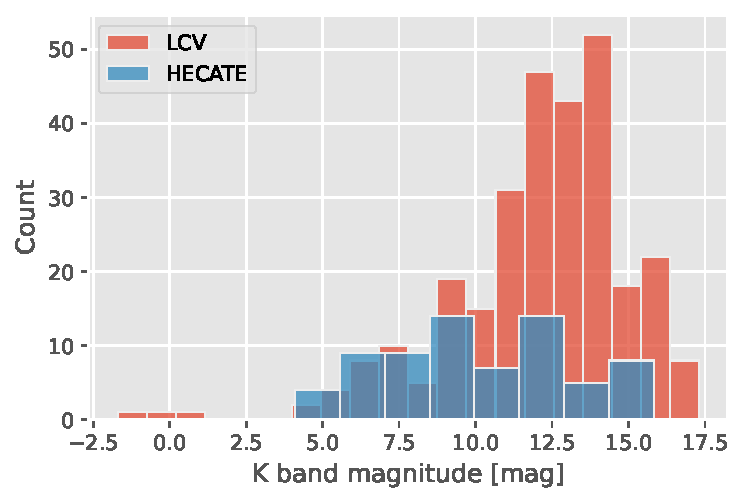
\includegraphics{compare_files/figure-pdf/cell-31-output-2.pdf}

\subsection{Luminosities}\label{luminosities}

\begin{longtable}[]{@{}cccc@{}}
\toprule\noalign{}
LCV & HECATE & Description & Pearson Correlation {[}-1,1{]} \\
\midrule\noalign{}
\endhead
\bottomrule\noalign{}
\endlastfoot
logKLum & logL\_K & & 0 \\
\end{longtable}

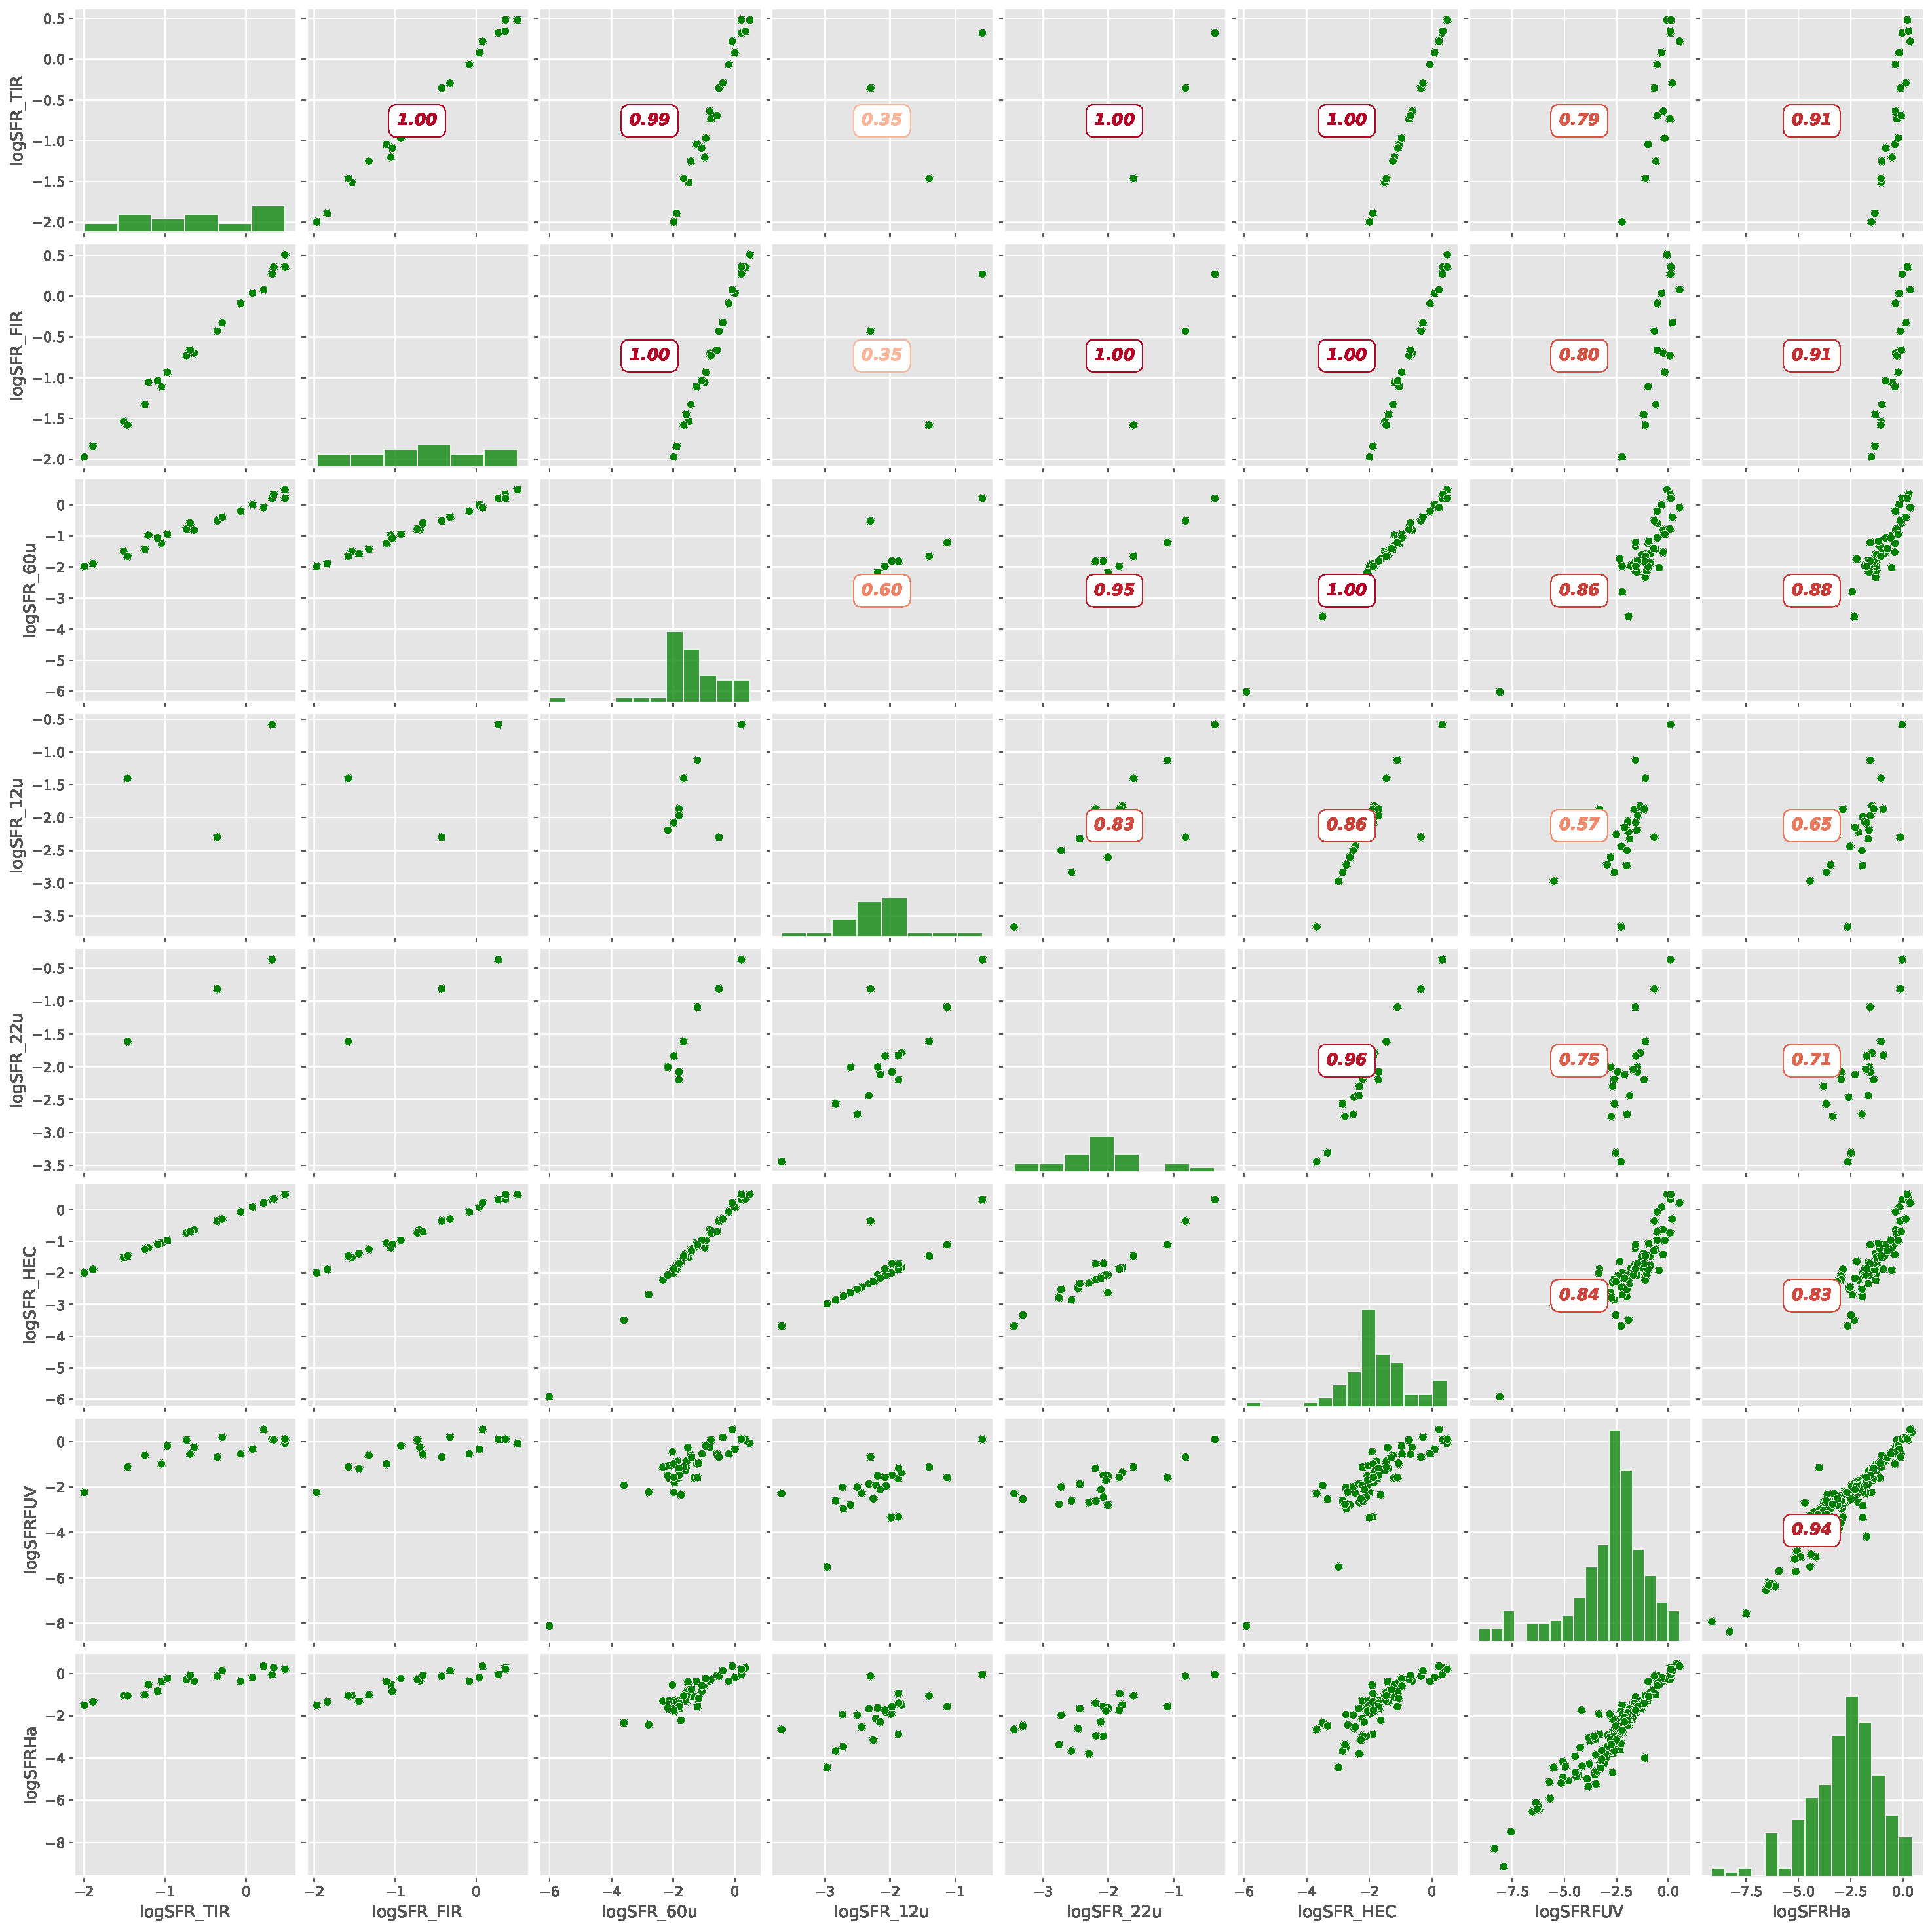
\includegraphics{compare_files/figure-pdf/cell-33-output-1.pdf}

\begin{longtable}[]{@{}llll@{}}
\toprule\noalign{}
& log(L\_K)\_\{LCV\}\$ & log(L\_K)\_\{HEC\} & Percentage Change
{[}\%{]} \\
\midrule\noalign{}
\endhead
\bottomrule\noalign{}
\endlastfoot
count & 287 & 70 & 70 \\
mean & 8 & 9 & -4 \\
std & 1 & 1 & 8 \\
min & 3 & 5 & -48 \\
50\% & 8 & 9 & -0 \\
max & 11 & 11 & 7 \\
\end{longtable}

\subsection{Magnitudes}\label{magnitudes}

\begin{longtable}[]{@{}
  >{\centering\arraybackslash}p{(\columnwidth - 6\tabcolsep) * \real{0.2466}}
  >{\centering\arraybackslash}p{(\columnwidth - 6\tabcolsep) * \real{0.2466}}
  >{\centering\arraybackslash}p{(\columnwidth - 6\tabcolsep) * \real{0.2466}}
  >{\centering\arraybackslash}p{(\columnwidth - 6\tabcolsep) * \real{0.2603}}@{}}
\toprule\noalign{}
\begin{minipage}[b]{\linewidth}\centering
LCV
\end{minipage} & \begin{minipage}[b]{\linewidth}\centering
HECATE
\end{minipage} & \begin{minipage}[b]{\linewidth}\centering
Description
\end{minipage} & \begin{minipage}[b]{\linewidth}\centering
Pearson Correlation {[}-1,1{]}
\end{minipage} \\
\midrule\noalign{}
\endhead
\bottomrule\noalign{}
\endlastfoot
mag\_B (with errors) & BT (with errors) & & 0 \\
Kmag & K & 2MASS band magnitude (both) & 0 \\
\end{longtable}

\subsubsection{B mag}

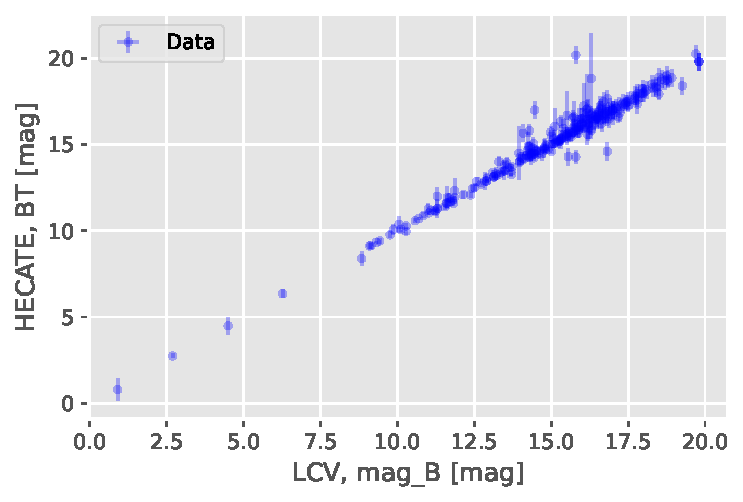
\includegraphics{compare_files/figure-pdf/cell-37-output-1.pdf}

\subsubsection{K mag}

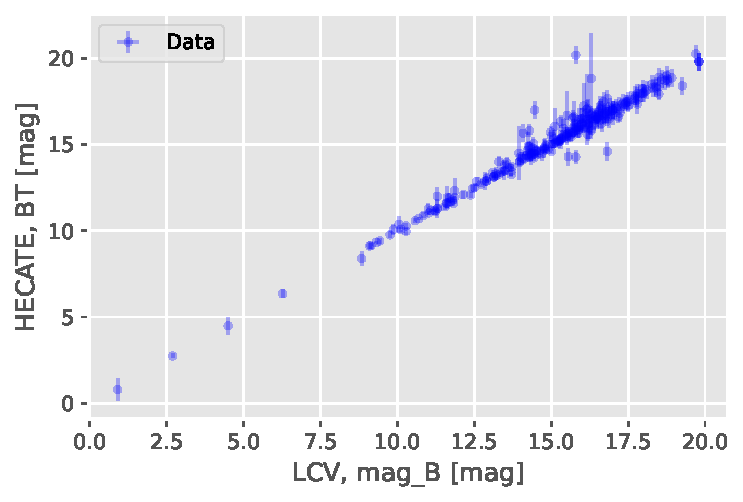
\includegraphics{compare_files/figure-pdf/cell-38-output-1.pdf}

\begin{longtable}[]{@{}lll@{}}
\toprule\noalign{}
& Percentage Change {[}\%{]} & Percentage Change, after 3 sigma clip
{[}\%{]} \\
\midrule\noalign{}
\endhead
\bottomrule\noalign{}
\endlastfoot
count & 70 & 70 \\
mean & -5 & -5 \\
std & 12 & 10 \\
min & -70 & -42 \\
50\% & -0 & -0 \\
max & 16 & 16 \\
\end{longtable}

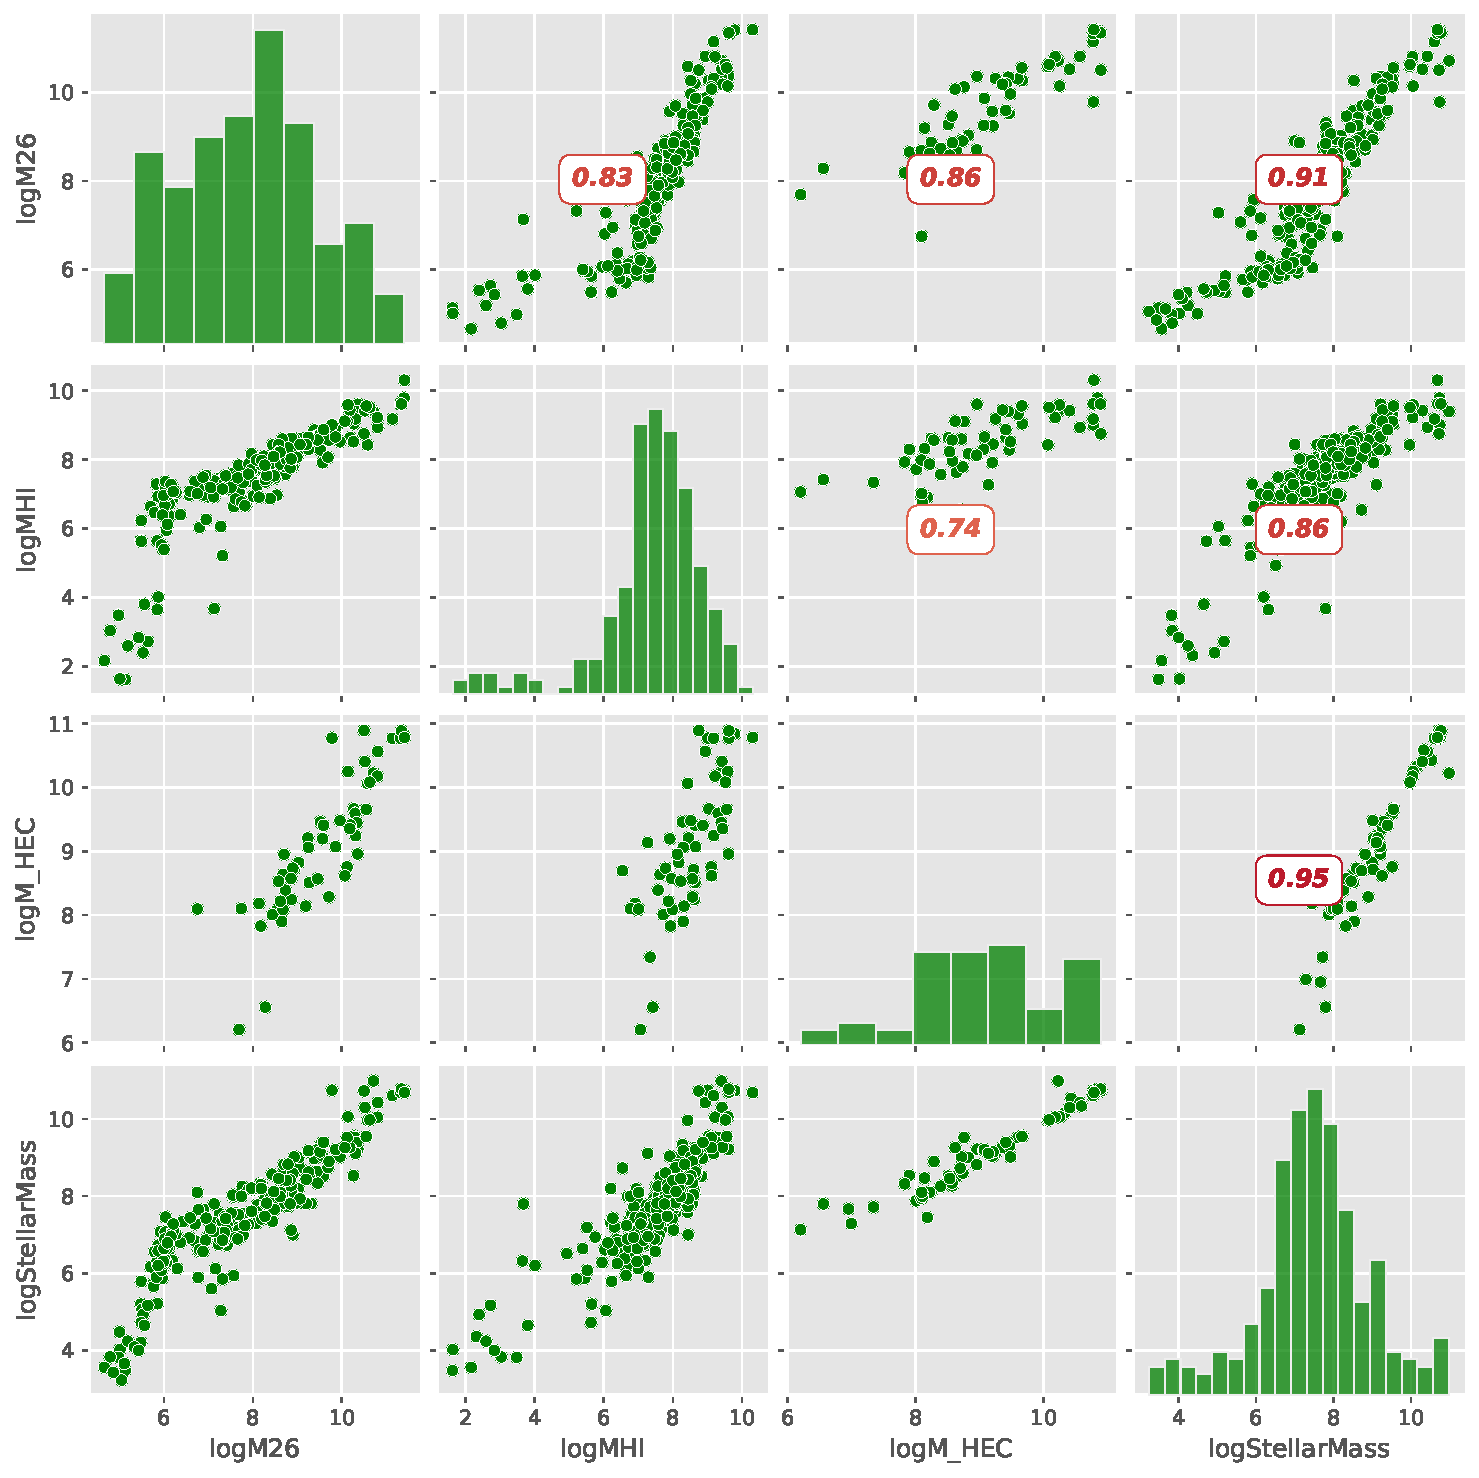
\includegraphics{compare_files/figure-pdf/cell-40-output-1.pdf}

{[}?{]}

\subsection{SFR}\label{sfr}

\begin{longtable}[]{@{}
  >{\centering\arraybackslash}p{(\columnwidth - 6\tabcolsep) * \real{0.2466}}
  >{\centering\arraybackslash}p{(\columnwidth - 6\tabcolsep) * \real{0.2466}}
  >{\centering\arraybackslash}p{(\columnwidth - 6\tabcolsep) * \real{0.2603}}
  >{\centering\arraybackslash}p{(\columnwidth - 6\tabcolsep) * \real{0.2466}}@{}}
\toprule\noalign{}
\begin{minipage}[b]{\linewidth}\centering
LCV
\end{minipage} & \begin{minipage}[b]{\linewidth}\centering
HECATE
\end{minipage} & \begin{minipage}[b]{\linewidth}\centering
Description
\end{minipage} & \begin{minipage}[b]{\linewidth}\centering
Count
\end{minipage} \\
\midrule\noalign{}
\endhead
\bottomrule\noalign{}
\endlastfoot
& logSFR\_TIR & Decimal logarithm of the total-infrared SFR estimate
{[}Msol/yr{]} & 21 \\
& logSFR\_FIR & Decimal logarithm of the far-infrared SFR estimate
{[}Msol/yr{]} & 22 \\
& logSFR\_60u & Decimal logarithm of the 60um SFR estimate {[}Msol/yr{]}
& 48 \\
& logSFR\_12u & Decimal logarithm of the 12um SFR estimate {[}Msol/yr{]}
& 26 \\
& logSFR\_22u & Decimal logarithm of the 22um SFR estimate {[}Msol/yr{]}
& 23 \\
& logSFR\_HEC & Decimal logarithm of the homogenised SFR estimate
{[}Msol/yr{]} & 73 \\
& logSFR\_GSW & Decimal logarithm of the SFR in GSWLC-2 {[}Msol/yr{]} &
0 \\
SFRFUV & & FUV derived integral star formation rate & 220 \\
SFRHa & & H\{alpha\} derived integral star formation rate & 223 \\
\end{longtable}

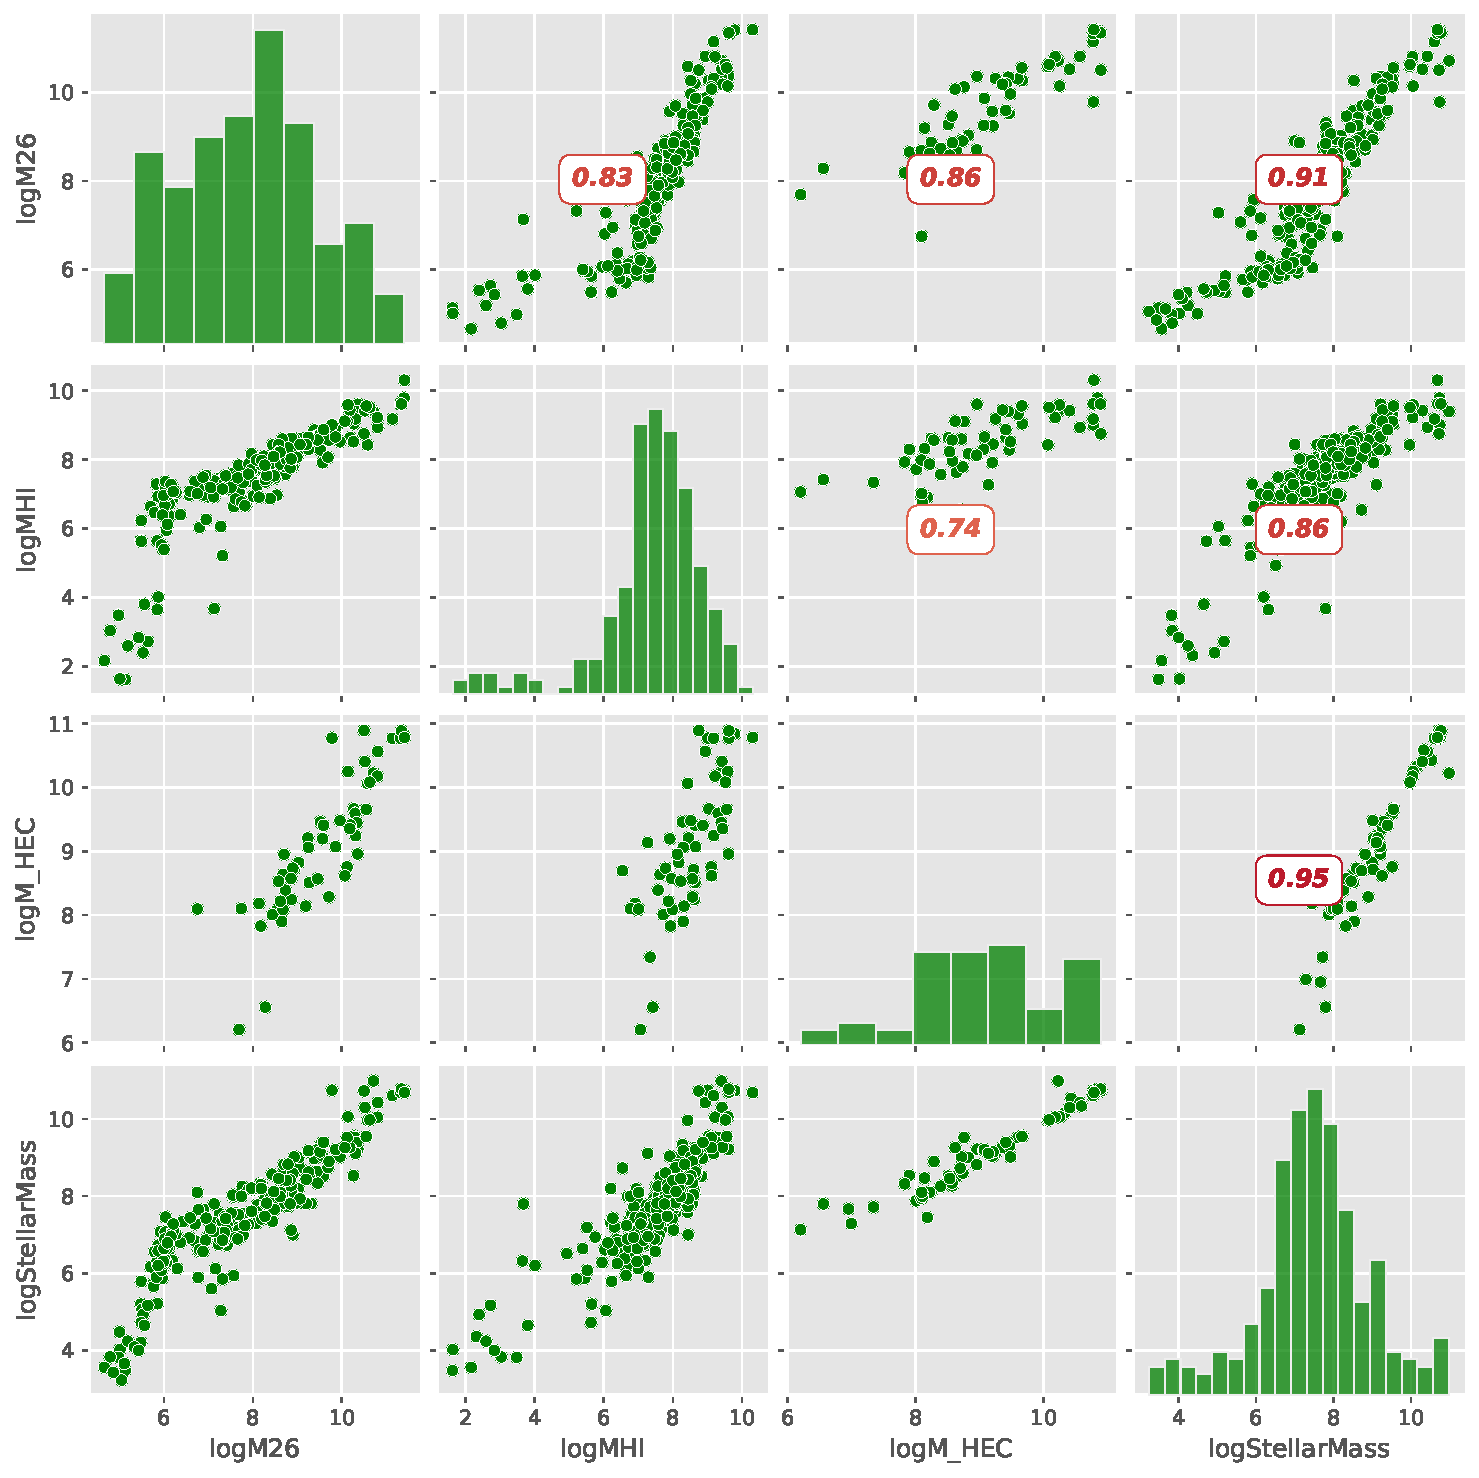
\includegraphics{compare_files/figure-pdf/cell-42-output-1.pdf}

\subsection{Masses}\label{masses}

\begin{longtable}[]{@{}
  >{\centering\arraybackslash}p{(\columnwidth - 6\tabcolsep) * \real{0.2500}}
  >{\centering\arraybackslash}p{(\columnwidth - 6\tabcolsep) * \real{0.2500}}
  >{\centering\arraybackslash}p{(\columnwidth - 6\tabcolsep) * \real{0.2500}}
  >{\centering\arraybackslash}p{(\columnwidth - 6\tabcolsep) * \real{0.2500}}@{}}
\toprule\noalign{}
\begin{minipage}[b]{\linewidth}\centering
LCV
\end{minipage} & \begin{minipage}[b]{\linewidth}\centering
HECATE
\end{minipage} & \begin{minipage}[b]{\linewidth}\centering
Description
\end{minipage} & \begin{minipage}[b]{\linewidth}\centering
Count
\end{minipage} \\
\midrule\noalign{}
\endhead
\bottomrule\noalign{}
\endlastfoot
logM26 & & Log mass within Holmberg radius & 233 \\
logMHI & & Log mass within Holmberg radius & 233 \\
& logM\_HEC & Decimal logarithm of the stellar mass {[}Msol{]} & 64 \\
& logM\_GSW & Decimal logarithm of the stellar mass in GSWLC-2
{[}Msol{]} & 0 \\
logStellarMass & & Stellar Mass from \(M_*/L=0.6\) & 287 \\
\end{longtable}

\subsubsection{Stellar Masses Comparison}

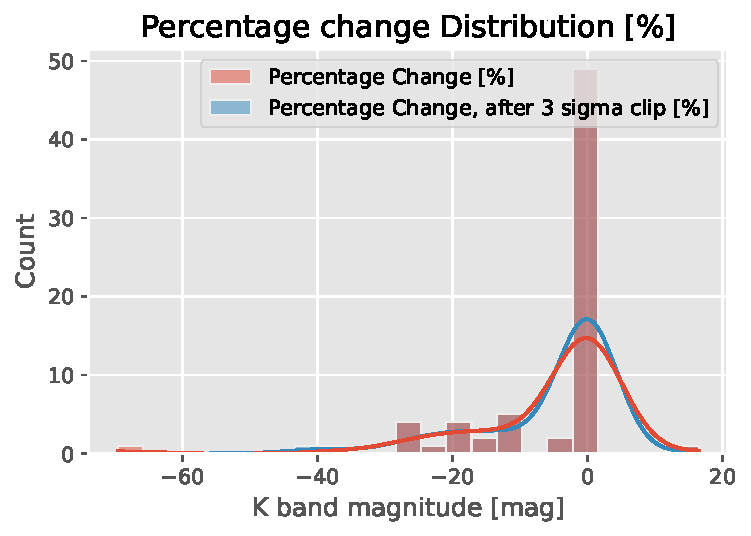
\includegraphics{compare_files/figure-pdf/cell-44-output-1.pdf}

\begin{longtable}[]{@{}ll@{}}
\toprule\noalign{}
& Percantage Change {[}\%{]} \\
\midrule\noalign{}
\endhead
\bottomrule\noalign{}
\endlastfoot
count & 64 \\
mean & -1 \\
std & 5 \\
min & -19 \\
50\% & 1 \\
max & 9 \\
\end{longtable}

\subsubsection{Heatmap}

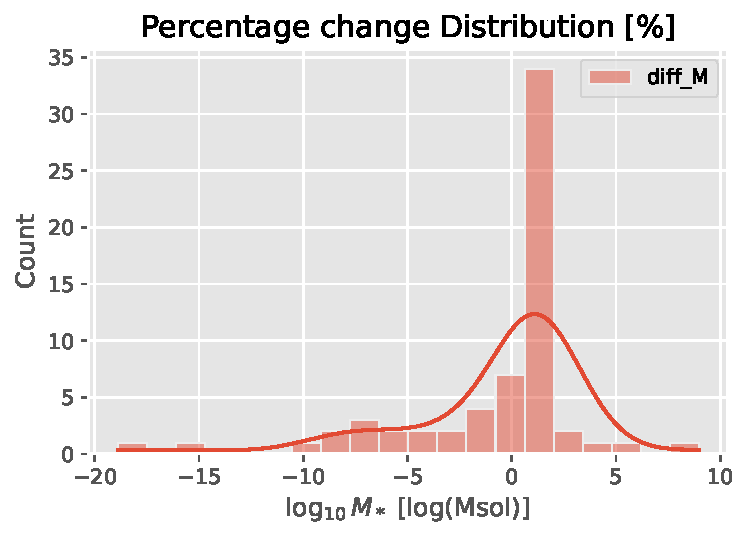
\includegraphics{compare_files/figure-pdf/cell-47-output-1.pdf}

\phantomsection\label{refs}
\begin{CSLReferences}{1}{0}
\bibitem[\citeproctext]{ref-karachentsevSTARFORMATIONPROPERTIES2013a}
Karachentsev, Igor D., and Elena I. Kaisina. 2013. {``{STAR FORMATION
PROPERTIES IN THE LOCAL VOLUME GALAXIES VIA Hα AND FAR-ULTRAVIOLET
FLUXES}.''} \emph{AJ} 146 (3): 46.
\url{https://doi.org/10.1088/0004-6256/146/3/46}.

\bibitem[\citeproctext]{ref-karachentsevUPDATEDNEARBYGALAXY2013}
Karachentsev, Igor D., Dmitry I. Makarov, and Elena I. Kaisina. 2013.
{``{UPDATED NEARBY GALAXY CATALOG}.''} \emph{AJ} 145 (4): 101.
\url{https://doi.org/10.1088/0004-6256/145/4/101}.

\bibitem[\citeproctext]{ref-kovlakasHeraklionExtragalacticCatalogue2021}
Kovlakas, K., A. Zezas, J. J. Andrews, A. Basu-Zych, T. Fragos, A.
Hornschemeier, K. Kouroumpatzakis, B. Lehmer, and A. Ptak. 2021. {``The
{Heraklion Extragalactic Catalogue} ({HECATE}): A Value-Added Galaxy
Catalogue for Multimessenger Astrophysics.''} \emph{Monthly Notices of
the Royal Astronomical Society} 506 (September): 1896--1915.
\url{https://doi.org/10.1093/mnras/stab1799}.

\end{CSLReferences}



\end{document}
